

%----------------------------------------------------------------------------------------
%	PACKAGES AND DOCUMENT CONFIGURATIONS
%----------------------------------------------------------------------------------------

\documentclass[a4paper,12pt]{article}
\usepackage[margin=0.9in]{geometry}
\usepackage{siunitx} % Provides the \SI{}{} and \si{} command for typesetting SI units
\usepackage{graphicx} % Required for the inclusion of images
\usepackage{subfigure}
\usepackage{multirow}
\usepackage{amsmath} % Required for some math elements 
\usepackage{indentfirst}
\usepackage{times} % Uncomment to use the Times New Roman font
\usepackage{appendix}
\usepackage{verbatim}

%----------------------------------------------------------------------------------------
%	DOCUMENT INFORMATION
%----------------------------------------------------------------------------------------
\title{ \rule{\textwidth}{0.3mm} \\UM–SJTU JOINT INSTITUTE \\ PHYSICS LABORATORY \\ (VP141) \\ \rule{\textwidth}{0.3mm} \\ [30 mm]  \Large{Laboratory Report} \\[5 mm]  Exercise 2 \\[1 mm] Measurement of Fluid Viscosity\\[15 mm]} % Title
\author{Cao Zhiyuan} % Author name
\date{\today} % Date for the report

\begin{document}
\scshape

\maketitle % Insert the title, author and date

\begin{center}
\begin{tabular}{l l l}
\\[16 mm]
Partners:  \\
Name: Cao Zhiyuan & ID: 518370910030 & Group: 14 \\
~\\
Date Performed:\\
July 19, 2019\\
\end{tabular}
\end{center}
\thispagestyle{empty}


\newpage


\small\tableofcontents
\thispagestyle{empty}


\newpage

%----------------------------------------------------------------------------------------
%	SECTION 1
%----------------------------------------------------------------------------------------

\setcounter{page}{1}
\upshape
\section{\textsc{Introduction}}
Viscosity is known to be one of the most indispensable characteristics for fluid in hydromechanics, which numerically describe the resistance an object will encounter when moving in a liquid. The objective of lab 2 is to learn and be acquaint with viscosity and the experimental methods to measure it. In this experiment, the method we apply is Stokes' method, which is widely used in analysing liquid with high viscosity.

%----------------------------------------------------------------------------------------
%	SECTION 2
%----------------------------------------------------------------------------------------

\section{\textsc{Theoretical background}}
When an object is moving in a fluid, it is exposed to a drag force whose direction is opposite to the direction of velocity. The magnitude of the drag force is influenced by properties of the object (shape and speed), as well as the internal friction of the fluid. To quantify the internal friction, we use a parameter $\eta$ called viscosity coefficient.
\par To further study the problem, we set up a basic model assuming that the object is spherical. Then, when the object is falling in the fluid, it is often acted upon three forces: the viscous force $F_v$, the buoyancy force $F_b$, and the gravitational force $G$. Since the three forces are in balance, we have:
\begin{equation}
F_v + F_b = G
\end{equation}
\par Then, we calculate these forces successively. First, for the drag force, we use the following formula: 
\begin{equation}
F_v = 6\pi \eta vR
\end{equation}
where $\eta$ is the drag coefficient, $R$ is the radius of the object, and $v$ is its velocity. The buoyancy force $F_b$ can be expressed as
\begin{equation}
F_b = \frac{4}{3}\pi R^3 \rho g
\end{equation}
where $\rho$ refers to the density of fluid, and $g$ is gravitational acceleration. And the magnitude of gravitational force G is
\begin{equation}
G = mg
\end{equation}
where $m$ is the mass of the object.
\par Since the system is in balance, the net force is zero and eventually the object will move in a constant speed. The speed $v_t$ is known as terminal speed. From Eq.(1), (2), (3) and (4), the drag coefficient can be expressed in terms of $g$, $R$, $\rho$, $m$, and $v_t$:
\begin{equation}
\eta = \frac{mg-\frac{4}{3}\pi R^3\rho g}{6\pi v_tR}
\end{equation}
\par After the motion reaches its terminal state, the terminal speed can be rewritten as $v_t = s/t$. Hence, the drag coefficient can be rewritten as:
\begin{equation}
\eta = \frac{mgt-\frac{4}{3}\pi R^3\rho gt}{6\pi sR}
\end{equation}
where $s$ is the distance travelled after reaching the terminal state, and $t$ is the corresponding time.
\par However, in our experiment, due to the restriction of container, some boundary effects should be considered. Hence, Eq.(2) ought to be modified. The newly calculated drag force is
\begin{equation}
F_v = 6\pi \eta vR (1+2.4\frac{R}{R_c})
\end{equation}
where $R_c$ is the radius of the cylindrical container.
\par Accordingly, the drag coefficient can be rewritten as 
\begin{equation}
\eta = \frac{mgt-\frac{4}{3}\pi R^3\rho gt}{6\pi sR(1+2.4\frac{R}{R_c})}
\end{equation}
\par Since the length of the container isn't infinite, further correction may be introduced about it.
%----------------------------------------------------------------------------------------
%	SECTION 3
%----------------------------------------------------------------------------------------
\section{\textsc{Apparatus}}
In this experiment, the most important device we use is Stokes’ viscosity measurement device, which has been shown in Figure 1. The device will be filled with highly viscous caster oil, and a small metal ball will fall in the device with its motion being studied. Besides, since many other physical quantities ought to be measured, devices also include thermometer, micrometer, densimeter, stopwatch, calliper, and electronic scales. Some detailed information regarding their uncertainties are listed in Table 1.

\begin{figure}[h] 
    \centering
    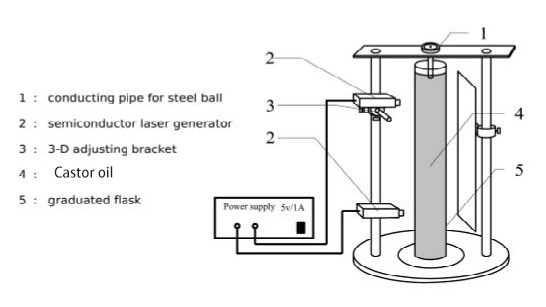
\includegraphics[width=0.5\textwidth]{Fig1} 
    \caption{Stokes’ viscosity measurement apparatus \cite{labmanual}} 
\end{figure}

\begin{table}[h]
\begin{center}
\begin{tabular}{cccc}
\hline
Name of the instrument & Measured quantities & Range & Uncertainty\\
\hline
Thermometer & Temperature & $0.2[^{\circ}C]$ & $\pm 0.1[^{\circ}C]$\\
Micrometer & Diameter of metal ball & $0.01 [mm]$ & $\pm 0.005 [mm]$\\
Densimeter & Density of caster oil & $0.001 [g/cm^3]$ & $\pm 0.0005 [g/cm^3]$\\
Stopwatch & Time & $0.01[s]$ & $\pm 0.01 [s]$\\
Calliper & Diameter of the flask & $0.02 [mm]$ & $\pm 0.02 [mm]$\\
Electronic scale & Mass of the metal ball & $0.001 [g]$ & $\pm 0.001 [g]$\\
Ruler & Distance between two laser beams & $1 [mm]$& $\pm 0.5 [mm]$\\
\hline
\end{tabular}
\end{center}
\caption{Table of details in the Instruments}
\end{table}

%----------------------------------------------------------------------------------------
%	SECTION 4
%----------------------------------------------------------------------------------------

\section{\textsc{Procedure}}
\subsection{\textsc{Adjustments of Stokes’ viscosity measurement apparatus}}
We begin our experiment by adjusting the Stokes’ viscosity measurement apparatus. First, we rotate the knobs on the base to adjust the plumb to make sure that its center is the same as the base's center so that the platform is horizontal. Second, we turn on the two laser beams, and with the help of ruler, make some adjustments to let them shot on the plumb line. Third, we place the flask in the middle of the base. After that, we put a guiding pipe in front of the flask to be prepared for falling the balls. And finally, we plug in the metal ball in the pipe to see whether it will pass through the laser beams and keep out the light of laser. If not, repeat from step 1.
\subsection{\textsc{Measurement of the terminal speed of the ball}}
Then, we measure the terminal speed of the ball. To begin with, we use ruler to measure the vertical distance $s$ between the two leaser beams for three times. Then, we put a metal ball into the fluid and record the time $t$ spent on falling between the two laser beams. After recording the values for six times to reduce the uncertainty, we are able to use $v = s/t$ to obtain the terminal speed of the meta ball.
\subsection{\textsc{Measurement of the remaining physical quantities and calculation the viscosity coefficient $\eta$}}
In this section, we measure the remaining quantities. To begin with, we measure the density of caster oil with the help of densimeter. Then, we measure the temperature of the oil with the help of thermometer. After that, we use calliper to measure the flask's inner diameter and micrometer to measure the diameter of the metal ball. Eventually, we find out he viscosity coefficient $\eta$ after plug in the parameters into Eq.(8).

%----------------------------------------------------------------------------------------
%	SECTION 5
%----------------------------------------------------------------------------------------

\section{\textsc{Result}}
%\subsection{\textsc{Distance between two laser beams}}
By measuring the distance between the two laser beams for three times, we obtain the result in Table 2:

\begin{table}[h]
\begin{center}
\begin{tabular}{|c|c|c|c|c|c|}
\hline
\multicolumn{6}{|c|}{distance $x [mm] \pm 0.5 [mm]$} \\
\hline
$x_{A,1}$ & ~~~~~57~~~~~ & $x_{B,1}$ & ~~~~178~~~~ & $S_1$ &~~~121~~~~\\
$x_{A,2}$ & 58 & $x_{B,2}$ & 178 & $S_2$ & 120\\
$x_{A,3}$ & 57 & $x_{B,3}$ & 178 & $S_3$ & 121\\
\hline
\end{tabular}
\caption{Data table for distance between two laser beams}
\end{center}
\end{table}

Then, we are able to calculate the average value for $x_A$ and $x_B$ respectively.
\begin{center}
$\displaystyle x_A = \frac{1}{3}\sum_{i=1}^3x_{A,i} = 57.3 [mm] \pm  1.5[mm] $~~~~~~$\displaystyle u_{rX_A} = 3\%$
\\
$\displaystyle x_B = \frac{1}{3}\sum_{i=1}^3x_{B,i} = 178.0 [mm] \pm  0.5[mm] $~~~~~~$\displaystyle u_{rX_B} = 0.3\%$
\end{center}

The distance between the two laser beams can be calculated by using $S = x_B - x_A$. Its relative uncertainty can also be calculated at the same time (The detailed calculations are shown in Appendix A.1.1):
\begin{center}
$\displaystyle S = x_B - x_A = 120.7 [mm] \pm 1.6 [mm] $~~~~~~$\displaystyle u_{rS} = 1.3 \%$
\end{center}

\par After measuring the distance, we use stopwatch to record the time spent on passing through these two points. The data are collected in Table 3:

\begin{table}[h]
\begin{center}
\begin{tabular}{|c|c|c|c|}
\hline
\multicolumn{4}{|c|}{time $t [s] \pm 0.01 [s]$} \\
\hline
$t_1$ & ~~~5.67~~~ & $t_4$ & ~~~5.74~~~~\\
$t_2$ & 5.71 & $t_5$ & 5.71 \\
$t_3$ & 5.74 & $t_6$ & 5.74 \\
\hline
\end{tabular}
\caption{Data table for time measurement}
\end{center}
\end{table}

Then, the average value and its relative uncertainty are calculated based on the data in Table 3 (The detailed calculations are shown in Appendix A.1.2):
\begin{center}
$\displaystyle t = \frac{1}{6}\sum_{i=1}^6t_i = 5.72 [s] \pm 0.03 [s]$~~~~~~$\displaystyle u_{rt} = 0.5 \%$
\end{center}

\par The diameter of the metal ball is measured by micrometer, and the data has been recorded in Table 4.

\begin{table}[h]
\begin{center}
\begin{tabular}{|c|c||c|c|}
\hline
\multicolumn{4}{|c|}{diameter $d [mm] \pm 0.005 [mm]$} \\
\hline
$d_1$ & ~~~~1.99~~~~ & $d_6$ & ~~~~1.99~~~~~\\
$d_2$ & 1.99 & $d_7$ & 2.00 \\
$d_3$ & 2.00 & $d_8$ & 1.99 \\
$d_4$ & 1.99 & $d_9$ & 1.99 \\
$d_5$ & 1.99 & $d_{10}$ & 1.99 \\
\hline
\end{tabular}
\caption{Data table for diameter of metal ball}
\end{center}
\end{table}

Then, the average value and its relative uncertainty are calculated based on the data in Table 4 (The detailed calculations are shown in Appendix A.1.3):
\begin{center}
$\displaystyle d = \frac{1}{10}\sum_{i=1}^{10}d_i = 1.990 [mm] \pm 0.006 [mm]$~~~~~~$\displaystyle u_{rd} = 0.3 \%$
\end{center}

\par The inner diameter of the flask is measured by calliper, and the data has been recorded in Table 5.

\begin{table}[h]
\begin{center}
\begin{tabular}{|c|c||c|c|}
\hline
\multicolumn{4}{|c|}{diameter $D [mm] \pm 0.02 [mm]$} \\
\hline
$D_1$ & ~~~63.08~~~ & $D_4$ & ~~~63.10~~~~\\
$D_2$ & 63.00 & $D_5$ & 63.12 \\
$D_3$ & 63.12 & $D_6$ & 63.06 \\
\hline
\end{tabular}
\caption{Data table for inner diameter of the flask}
\end{center}
\end{table}

Then, the average value and its relative uncertainty are calculated based on the data above (The detailed calculations are shown in Appendix A.1.4):
\begin{center}
$\displaystyle D = \frac{1}{6}\sum_{i=1}^{6}D_i = 63.08 [mm] \pm 0.05 [mm]$~~~~~~$\displaystyle u_{rD} = 0.09 \%$
\end{center}

\par The other remaining physical quantities and their uncertainties are shown in Table 6 (Detailed calculations are shown in Appendix A.2):

\begin{table}[h]
\begin{center}
\begin{tabular}{|c||c|c|}
\hline
density of the castor oil $\rho$ & $0.955 [g/cm^3] \pm 0.0005 [g/cm^3]$ & $u_{r\rho} = 0.05\%$ \\
mass of 40 metal balls $m$& $1.317 [g] \pm 0.001 [g]$ & $u_{rm} = 0.04\%$ \\
temperature in the lab $T$ & $28.2[^{\circ}C] \pm 0.1 [^{\circ}C]$ & $u_{rT} = 0.4\%$ \\
gravitational acceleration in the lab $g$ & $9.81 [m/s^2]$ & /\\
\hline
\end{tabular}
\caption{Data table for other physical parameters}
\end{center}
\end{table}

\par Finally, based on the above data, the viscosity coefficient $\eta$ can be calculated using Eq.(8):
\begin{center}
$\displaystyle \eta = \frac{\frac{1}{40}mgt-\frac{4}{3}\pi R^3\rho gt}{6\pi sR(1+2.4\frac{R}{R_c})} = \frac{\frac{1}{40}mgt-\frac{1}{6}\pi d^3\rho gt}{3\pi Sd(1+2.4\frac{d}{D})} = 0.668 \pm 0.010[Pa \cdot s]$
\end{center}
\begin{center}
$u_{r\eta} = 1.5 \%$
\end{center}

%----------------------------------------------------------------------------------------
%	SECTION 5.2
%----------------------------------------------------------------------------------------
\newpage
\section{\textsc{Discussion}}
In this lab, we generally deal with how to measure the viscosity coefficient of a fluid. Our experimental value of viscosity coefficient $\eta$ is 0.668 Pa·s with a relative uncertainty $1.5\%$. According to the data on website, the viscosity of oil in 20 $^{\circ} C$ is 800$cP$ (0.8 Pa·s), which is in the same order of magnitude compared with the final result we obtain in the lab\cite{ct1}. The deviation from theoretical value can be calculated as:
\begin{center}
$\displaystyle D = \frac{|\eta_{lab}-\eta_{theo}|}{\eta_{theo}} = 16.5 \%$
\end{center}
Also, the viscosity coefficient of water is $1*10^{-3}$ Pa·s\cite{ct3}. It corresponds with our common sense that the caster oil has a larger viscosity coefficient compared with water. However, there are still many places which need to be paid attention to. Otherwise some large errors is likely to occur.
\par To figure out the what factors lead to high errors, we find clarify some assumptions in our lab. To begin with, in our lab we assume that the object we release in the caster oil is completely spherical, which allows us to use Eq.(2) in our lab. Nevertheless, the ball is so small, and it must not be a complete spherical object. Thus possibly high errors will occur. Besides, in this lab, when we measure the velocity of the ball, we have already assumed that the ball has reaches its terminal speed without testing it. In other words, the velocity of the ball may still change after it reaches the first laser beam, which may lead to high errors.
\par Furthermore, there are also some mistakes in procedures which may lead to errors. First, when we place the flask containing caster oil, the light may be refracted, resulting in the change of the distance between two laser beams. Second, the length of the container is not infinite, and some modifications can be done further to Eq.(7) and Eq.(8) with respect to the height of the flask $H$.
\par Hence, now we discuss how to improve the procedure to minimize the uncertainty. To begin with, speaking of the assumption of whether the ball has reached a constant terminal speed, we can add three more laser beams (with the same interval distance between each two of them) in front of the previous ones. And we check time the ball spent on passing through the three successive laser beams. If the time is the same, it means that the ball has already reached its terminal velocity. And thus we can begin with our original procedure. Besides, in terms of the influence of the height of the flask, we can take into consideration the influence of it. In other words, Eq.(7) turns into:
\begin{center}
$F_v = 6\pi \eta vR (1+2.4\frac{R}{R_c})(1+1.6\frac{R}{H})$
\end{center}
where $H$ is the height of the flask\cite{ct2}. In this way, our result will be much closer to the actual value.
\par There may still be some factors like the unstability of temperature of the caster oil. Nevertheless, it's nearly impossible for us to exclude everything that may lead to errors. Hence, if we fulfil the factors in Discussion part, our uncertainty of result is sure to be in a satisfactory value.

\section{\textsc{Conclusion}}
In conclusion, in this lab, we apply Stokes’ method to find out the viscosity by assuming that the object is spherical and it has reached its terminal speed when begin measured. As a result, the value we calculated lastly is 0.668 Pa·s, with a relative uncertainty $1.5\%$. And the deviation from theoretical value is $22\%$. The value of viscosity coefficient is in the same order of magnitude compared with the theoretical value and corresponds to our common sense. Generally speaking, the experiment is successful for finding out the viscosity coefficient. 
\par Furthermore, if we want to revise the experiment to make the result closer to the actual one, we can do the following adjustments. To begin with, we check that the ball has already reached a constant speed before measuring its velocity. Besides, we take into consideration the influence of the height of the flask on the result and modify the formula for calculating viscosity coefficient. As an outlook, it would be better if the influence of temperature can be studied for future experiment.

%----------------------------------------------------------------------------------------
%	SECTION 6
%----------------------------------------------------------------------------------------

\begin{appendices} 
      \section{\textsc{Measurement uncertainty analysis}} 
      \subsection{\textsc{Uncertainty of Multiple Measurements}}
      In this experiment, we measured a variety of data by multiple measurements. The detailed calculations are shown below:
      \subsubsection{\textsc{Uncertainty of distance between two laser beams}}
      For the vertical distance, we first calculate the average value of $x_{A}$ and $x_{B}$:
      \begin{center}
      $\displaystyle\bar{x_A} = \frac{1}{3}\sum_{i=1}^3x_{A,i} = 57.3 [mm]$
      \end{center}
      Then, we calculate the standard deviation:
      \begin{center}
      $\displaystyle S_{x_A} = \sqrt{\frac{1}{2}\sum_{i=1}^3(x_{A,i} - \bar{x_A})^2} = 0.6 [mm]$
      \end{center}
      Hence, we obtain $\Delta_{A,x_{A}}$:
      \begin{center}
      $\displaystyle\Delta_{A,x_A} = S_{x_A} \frac{t_{0.95}}{\sqrt{3}} = 2.48*0.6 = 1.4 [mm]$
      \end{center}
      Because of the limitation of instrument, our $\Delta_{B,x_A} = 0.5 [mm]$. Hence, the overall uncertainty is:
      \begin{center}
      $\Delta_{x_A} = \sqrt{\Delta_{A,x_A}^2 + \Delta_{B,x_A}^2} = \sqrt{1.4^2 + 0.5^2} = 1.5 [mm]$
      \end{center}
      with a corresponding relative uncertainty
      \begin{center}
      $\displaystyle u_{rX_A} = \frac{u_{x_A}}{\bar{x_A}} = \frac{1.5}{57.3}*100\% \approx 3\%$
      \end{center}
      \par Similarly, we obtain $x_B$ by the same procedure:
        \begin{center}
      $\displaystyle\bar{x_B} = \frac{1}{3}\sum_{i=1}^3x_{B,i} = 178 [mm]$ \\[2 mm]
      $\displaystyle S_{x_B} = \sqrt{\frac{1}{2}\sum_{i=1}^3(x_{B,i} - \bar{x_B})^2} = 0 [mm]$ \\[2 mm]
      $\displaystyle\Delta_{A,x_B} = S_{x_B} \frac{t_{0.95}}{\sqrt{3}} = 2.48*0 = 0 [mm]$\\[2 mm]
      $\Delta_{x_B} = \sqrt{\Delta_{B,x_B}^2 + \Delta_{B,x_B}^2} = \sqrt{0^2 + 0.5^2} = 0.5 [mm]$ \\[2 mm]
      $\displaystyle u_{rX_B} = \frac{u_{x_B}}{\bar{x_B}} = \frac{0.5}{178}*100\% \approx 0.3\%$
      \end{center}
      \par Eventually, we are able to calculate the distance $S$ by the equation $S = x_B - x_A$.
      Since we have
      \begin{center}
      $\displaystyle \frac{\partial S}{\partial{x_A}} = -1 $\\ [2 mm]
      $\displaystyle \frac{\partial S}{\partial{x_B}} = 1 $
      \end{center}
      we can further obtain:
      \begin{center}
      $\displaystyle u_S = \sqrt{(\frac{\partial S}{\partial{x_A}})^2(x_A)^2 + (\frac{\partial S}{\partial{x_B}})^2(x_B)^2} = \sqrt{1.5^2 + 0.5^2} = 1.6 [mm]$
      \end{center}
      with a corresponding relative uncertainty 
      \begin{center}
      $\displaystyle u_{rS} = \frac{u_S}{\bar{S}} = \frac{1.6}{120.7} * 100\% \approx 1.3 \%$
      \end{center}
      
      \subsubsection{\textsc{Uncertainty of time measurement}}
      For the time measurement, we first calculate its average value:
      \begin{center}
      $\displaystyle\bar{t} = \frac{1}{6}\sum_{i=1}^6t_i = 5.72 [s]$
      \end{center}
      Then, we calculate the standard deviation:
      \begin{center}
      $\displaystyle S_t = \sqrt{\frac{1}{5}\sum_{i=1}^6(t_i - \bar{t})^2} = 0.03 [s]$
      \end{center}
      Hence, we obtain $\Delta_{A,t}$:
      \begin{center}
      $\displaystyle\Delta_{A,t} = S_t \frac{t_{0.95}}{\sqrt{6}} = 1.05*0.03 = 0.03 [s]$
      \end{center}
      Because of the limitation of instrument, our $\Delta_{B,t} = 0.01 [s]$. Hence, the overall uncertainty is:
      \begin{center}
      $\Delta_t = \sqrt{\Delta_{A,t}^2 + \Delta_{B,t}^2} = \sqrt{0.03^2 + 0.01^2} \approx 0.03 [s]$
      \end{center}
      with a corresponding relative uncertainty
      \begin{center}
      $\displaystyle u_{rt} = \frac{u_t}{\bar{t}} = \frac{0.03}{5.72}*100\% \approx 0.5\%$
      \end{center}      
      
      \subsubsection{\textsc{Uncertainty of diameter of metal ball}}
      For the time measurement, we first calculate its average value:
      \begin{center}
      $\displaystyle\bar{d} = \frac{1}{10}\sum_{i=1}^{10}d_i = 1.990 [mm]$
      \end{center}
      Then, we calculate the standard deviation:
      \begin{center}
      $\displaystyle S_d = \sqrt{\frac{1}{9}\sum_{i=1}^{10}(d_i - \bar{d})^2} = 0.004 [mm]$
      \end{center}
      Hence, we obtain $\Delta_{A,d}$:
      \begin{center}
      $\displaystyle\Delta_{A,d} = S_d \frac{t_{0.95}}{\sqrt{10}} = 0.715*0.004 = 0.003 [mm]$
      \end{center}
      Because of the limitation of instrument, our $\Delta_{B,d} = 0.005 [mm]$. Hence, the overall uncertainty is:
      \begin{center}
      $\Delta_d = \sqrt{\Delta_{A,d}^2 + \Delta_{B,d}^2} = \sqrt{0.003^2 + 0.005^2} \approx 0.006 [mm]$
      \end{center}
      with a corresponding relative uncertainty
      \begin{center}
      $\displaystyle u_{rd} = \frac{u_d}{\bar{d}} = \frac{0.006}{1.99}*100\% \approx 0.3\%$
      \end{center}      
      
      \subsubsection{\textsc{Uncertainty of inner diameter of the flask}}
      For the time measurement, we first calculate its average value:
      \begin{center}
      $\displaystyle\bar{D} = \frac{1}{6}\sum_{i=1}^{6}D_i = 63.08 [mm]$
      \end{center}
      Then, we calculate the standard deviation:
      \begin{center}
      $\displaystyle S_D = \sqrt{\frac{1}{5}\sum_{i=1}^{6}(D_i - \bar{D})^2} = 0.05 [mm]$
      \end{center}
      Hence, we obtain $\Delta_{A,D}$:
      \begin{center}
      $\displaystyle\Delta_{A,D} = S_d \frac{t_{0.95}}{\sqrt{6}} = 1.05*0.05 = 0.05 [mm]$
      \end{center}
      Because of the limitation of instrument, our $\Delta_{B,D} = 0.02 [mm]$. Hence, the overall uncertainty is:
      \begin{center}
      $\displaystyle \Delta_D = \sqrt{\Delta_{A,D}^2 + \Delta_{B,D}^2} = \sqrt{0.05^2 + 0.02^2} \approx 0.05 [mm]$
      \end{center}
      with a corresponding relative uncertainty
      \begin{center}
      $\displaystyle u_{rD} = \frac{u_D}{\bar{D}} = \frac{0.05}{63.08}*100\% \approx 0.09\%$
      \end{center}      
      
      \subsection{\textsc{Uncertainty of Single Measurements}}
      Since in this experiment many parameters are only measured once, their type-A uncertainties are always equal to 0, and thus the overall uncertainties are the type-B uncertainties which are limited by the resolution of instruments.
      \subsubsection{\textsc{Uncertainty of the density of the caster oil}}
      In this experiment, we use densimeter to measure the density of caster oil only once. Therefore the uncertainty is 
      \begin{center}
      $\displaystyle u_{\rho} = 0.0005 [g/cm^3]$
      \end{center}
      with a relative uncertainty 
      \begin{center}
      $\displaystyle u_{r\rho} = \frac{u_{\rho}}{\rho} = \frac{0.0005}{0.955} * 100\% \approx 0.05 \%$
      \end{center}
      \subsubsection{\textsc{Uncertainty of the mass of 40 metal balls}}
      In this experiment, we use electronic scale to measure the mass of 40 metal balls only once. Therefore the uncertainty is 
      \begin{center}
      $ \displaystyle u_{m} = 0.001 [g]$
      \end{center}
      with a relative uncertainty 
      \begin{center}
      $ \displaystyle u_{rm} = \frac{u_{m}}{m} = \frac{0.0005}{1.317} * 100\% \approx 0.04 \%$
      \end{center}
      \subsubsection{\textsc{Uncertainty of temperature in lab}}
      In this experiment, we use thermometer to measure the temperature in the lab only once. Therefore the uncertainty is 
      \begin{center}
      $ \displaystyle u_{T} = 0.1 [^{\circ}C]$
      \end{center}
      with a relative uncertainty 
      \begin{center}
      $ \displaystyle u_{rT} = \frac{u_{T}}{T} = \frac{0.1}{28.2} * 100\% \approx 0.4 \%$
      \end{center}
       \subsection{\textsc{Uncertainty of Indirect Measurements}}
      In this experiment, we figure out the viscosity coefficient indirectly by applying Eq.(8). We have the physical quantity $\eta$ which can be expressed in terms of $m$, $t$, $d$, $\rho$, $D$ and $S$. In other words, we have 
      \begin{center}
      $\displaystyle \eta(m,t,\rho,d,D,S) = \frac{\frac{1}{40}mgt-\frac{1}{6}\pi d^3\rho gt}{3\pi Sd(1+2.4\frac{d}{D})} = 0.668 Pa \cdot s$
      \end{center}
      \par Then, we calculate the partial derivatives respectively. The partial derivatives with respect to each parameter are shown below:
      \begin{center}
      $\displaystyle \frac{\partial \eta}{\partial m} = \frac{gt}{120\pi Sd(1+2.4\frac{d}{D})}$
      \end{center}
      %m's Pd.
      \begin{center}
      $\displaystyle \frac{\partial \eta}{\partial t} = \frac{\frac{1}{40}mg-\frac{1}{6}\pi d^3\rho g}{3\pi Sd(1+2.4\frac{d}{D})}$
      \end{center}
      %t's Pd.
      \begin{center}
      $\displaystyle \frac{\partial \eta}{\partial \rho} = -\frac{d^2gt}{18S(1+2.4\frac{d}{D})}$
      \end{center}
      %\rho's Pd.
       \begin{center}
      $\displaystyle \frac{\partial \eta}{\partial d} =  -\frac{d \rho g t}{6S(1+2.4\frac{d}{D})} -  \frac{(\frac{1}{40}mgt-\frac{1}{6}\pi d^3\rho gt)(3 + \frac{14.4d}{D})}{9\pi Sd^2(1+2.4\frac{d}{D})^2}$
      \end{center}
      %\d's Pd.
       \begin{center}
      $\displaystyle \frac{\partial \eta}{\partial D} = \frac{7.2(\frac{1}{40}mgt-\frac{1}{6}\pi d^3 \rho g t)}{9\pi S (D+2.4d)^2}$
      \end{center}
      %\D's Pd.
      \begin{center}
      $\displaystyle \frac{\partial \eta}{\partial S} = - \frac{\frac{1}{40}mgt-\frac{1}{6}\pi d^3\rho gt}{3\pi S^2d(1+2.4\frac{d}{D})}$
      \end{center}
      %S's Pd.
      \par Hence, the uncertainty of viscosity coefficient $u_{\eta}$ can be calculated as follows: 
      \begin{align*}
      \displaystyle u_{\eta} &= \sqrt{(\frac{\partial \eta}{\partial m})^2(u_m)^2 + (\frac{\partial \eta}{\partial t})^2({u_t})^2 + (\frac{\partial \eta}{\partial \rho})^2(u_\rho)^2 + (\frac{\partial \eta}{\partial d})^2(u_d)^2 + (\frac{\partial \eta}{\partial D})^2(u_D)^2 + (\frac{\partial \eta}{\partial S})^2(u_S)^2}\\
&=((\frac{gt}{120\pi Sd(1+2.4\frac{d}{D})})^2(u_m)^2 + (\frac{\frac{1}{40}mg-\frac{1}{6}\pi d^3\rho g}{3\pi Sd(1+2.4\frac{d}{D})})^2(u_t)^2 + (-\frac{d^2gt}{18S(1+2.4\frac{d}{D})})^2(u_\rho)^2 + 
\\
& (-\frac{d \rho g t}{6S(1+2.4\frac{d}{D})} -  \frac{(\frac{1}{40}mgt-\frac{1}{6}\pi d^3\rho gt)(3 + \frac{14.4d}{D})}{9\pi Sd^2(1+2.4\frac{d}{D})^2})^2(u_d)^2 + (\frac{7.2(\frac{1}{40}mgt-\frac{1}{6}\pi d^3 \rho g t)}{9\pi S (D+2.4d)^2})^2(u_D)^2 
\\
& + (- \frac{\frac{1}{40}mgt-\frac{1}{6}\pi d^3\rho gt}{3\pi S^2d(1+2.4\frac{d}{D})})^2(u_S)^2)^{\frac{1}{2}}
\\
& =0.010 [Pa\cdot s]
      \end{align*}
      with a relative uncertainty 
      \begin{center}
      $\displaystyle u_{r\eta} = \frac{u_\eta}{\eta} \approx 1.5\%$
      \end{center}
      
      \section{\textsc{Datasheet}} 
      See the last page.
  \end{appendices} 

%----------------------------------------------------------------------------------------
%	BIBLIOGRAPHY
%----------------------------------------------------------------------------------------

\begin{thebibliography}{9}
\bibitem{labmanual} Krzyzosiak, M. \& VP141 TA Group.
\textit{Exercise 5 - lab manual [rev 4].pdf}. 
2019.
\bibitem{ct1} https://www.quora.com/What-is-the-value-of-the-coefficient-of-the-viscosity-of-castor-oil
\bibitem{ct2} https://wenku.baidu.com/view/4e6b8e1d01f69e31433294dc.html?from=search
\bibitem{ct3} https://wenku.baidu.com/view/d51d188b88eb172ded630b1c59eef8c75fbf95d5.html
\end{thebibliography}



%----------------------------------------------------------------------------------------


\end{document}
